%%%%%%%%%%%%%%%%%%%%%%%%%%%%%%%%%%%%%%%%%%%%%%%%%%%%%%%%%%%%%%%%%%%%%%
% Lớp 11 | Đạo hàm | Các quy tắc đạo hàm
% Dạng 1D7?2-2: Đẳng thức có 𝑦và 𝑦′
% Số câu: 17  (sinh tự động bởi tach_cau.py; từ nay thầy sửa trực tiếp file này)
%%%%%%%%%%%%%%%%%%%%%%%%%%%%%%%%%%%%%%%%%%%%%%%%%%%%%%%%%%%%%%%%%%%%%%

%%%%%%%%%%%%%%%% TRẮC NGHIỆM 4 PHƯƠNG ÁN %%%%%%%%%%%%%%%%

% nguồn: Ok_TracNghiemLop11_Lan1
\begin{ex}%[1D7H2-2]%[ma:70a3e01e]
	Cho hàm số $y =  \sqrt{2x - x^2}$ có đạo hàm cấp hai. Mệnh đề nào sau đây đúng?
	\choice 
		{\True $y^3y''+1=0$} 
		 {$y'=\dfrac{1}{2\sqrt{2x-x^2}}$}
		{$y^2y''+y'=1$} 
		 {$y^2+y'-y''=1$}
	\loigiai{ 
	Với điều kiện $0<x<2$  ta có
	\begin{align*}
		&&y'=& \dfrac{(2x-x^2)'}{2\sqrt{2x-x^2}} =  \dfrac{2-2x}{2\sqrt{2x-x^2}} = \dfrac{1-x}{\sqrt{2x-x^2}}.\\
		&&y''=&  \dfrac{(1-x)'\sqrt{2x-x^2} - (1-x)\left(\sqrt{2x-x^2}\right)'}{2x-x^2}=\dfrac{-\sqrt{2x-x^2}-(1-x)\dfrac{1-x}{\sqrt{2x-x^2}}}{2x-x^2}\\
		&&=& \dfrac{-1}{(2x-x^2)\sqrt{2x-x^2}}\cdot 
	\end{align*}
	Do đó 
	\begin{align*}
		y^3y''+1 = \left(\sqrt{2x-x^2}\right)^3\dfrac{(-1)}{(2x-x^2)\sqrt{2x-x^2}}+1 =  -1 + 1 = 0.
	\end{align*}
	} 
\end{ex}

% nguồn: Ok_TracNghiemLop11_Lan1
\begin{ex}%[1D7H2-2]%[ma:47f67e10]
	Cho hàm số $f(x)=x^4-2x^2+1$. Tìm tất cả các giá trị của $x$ sao cho $f'(x)>0$. 
	\choice 
		{\True $x\in  (-1;0)\cup (1;+\infty)$}
		{$x\in  (-1;1)$}
		{$x\in (-\infty;-1)\cup (0;1)$} 
		 {$x\in \mathbb{R}$}
	 \loigiai{
		Ta  có $f'(x)=4x^3-4x=4x(x^2-1)$. \\
		$f'(x)>0 \Leftrightarrow  4x(x^2-1)>0$. \\
		Lập  bảng xét dấu:
		\begin{center}
			\begin{tikzpicture}
					\tkzTabInit[nocadre=false,lgt=2,espcl=2.1] 
						{$x$ /0.7,$4x$ /0.7,$x^2-1$ /0.7,$f'(x)$  /0.7}
						{$-\infty$,$-1$,$0$,$1$,$+\infty$} 
					 \tkzTabLine{,-,|,-,$0$,+,|,+,}
					 \tkzTabLine{,+,$0$,-,|,-,$0$,+,}
					 \tkzTabLine{,-,$0$,+,$0$,-,$0$,+,}
				\end{tikzpicture}
		\end{center}
	Từ bảng xét dấu  suy ra $f'(x)>0 \Leftrightarrow x\in (-1;0)\cup (1;+\infty)$.}
\end{ex}

% nguồn: Ok_TracNghiemLop11_Lan1
\begin{ex}%[1D7H2-2]%[ma:2372632e]
	Cho hàm số $y=\dfrac{1}{x+1+\ln x}$ với $ x>0$.  Khi đó $-\dfrac{y'}{y^2}$ bằng
	 \choice
		 {$\dfrac{x}{x+1}$}
		{\True $1+\dfrac{1}{x}$} 
		{$\dfrac{x}{1+x+\ln  x}$}
		{$\dfrac{x+1}{1+x+\ln  x}$}
	 \loigiai{
	$ y=\dfrac{1}{x+1+\ln x}\Rightarrow\dfrac{1}{y}=x+1+\ln  x\Rightarrow{\left(\dfrac{1}{y}\right)'}=\left(x+1+\ln x\right)'\Leftrightarrow-\dfrac{y'}{y^2}=1+\dfrac{1}{x}$.}
\end{ex}

% nguồn: Ok_Toan11_TracNghiem_Lan2
\begin{ex}%[1D7V2-2]%[ma:942740b9]
	Cho hai hàm số $f(x)$ và $g(x)$ đều có đạo hàm trên $\mathbb{R}$ và thỏa mãn $f^3(2-x)-2f^2(2+3x)+x^2\cdot g(x)+36x=0$, $\forall x\in\mathbb{R}$.  Tính $A=3f(2)+4f'(2)$.
	 \choice
		{$11$} 
		 {$13$}
		{$14$} 
		{\True $10$} 
	 \loigiai{
		 Theo giả thiết, ta có
		\begin{align*}
			f^3(2-x)-2f^2(2+3x)+x^2\cdot g(x)+36x=0,~\forall  x\in\mathbb{R}.\tag{1}
		\end{align*}
		Cho $x=0$, ta  được
		\begin{align*}
			f^3(2)-2f^2(2)=0\Leftrightarrow\hoac{&f(2)=0\\ &f(2)=2.}\tag{2} 
		\end{align*}
		Đạo  hàm hai vế của $(1)$, ta được
		\begin{align*}
			-3f^2(2-x)\cdot f'(2-x)-12f(2+3x)\cdot  f'(2+3x)+2x\cdot g(x)+x^2\cdot g'(x)+36=0,~\forall x\in\mathbb{R}.\tag{3}
		\end{align*}
		Cho $x=0$, ta  được
		\begin{align*}
			 -3f^2(2)\cdot f'(2)-12f(2)\cdot f'(2)+36=0\Leftrightarrow-3f(2)\cdot f'(2)\left[f(2)+4\right]+36=0. \tag{4}
		\end{align*}
		Từ $(4)$ suy ra $f(2)\neq0$, $f'(2)\neq0$. Do đó, từ $(2)$, ta  được $f(2)=2$. Khi đó, $(4)$ trở thành
		\begin{align*}
			 -3\cdot 2\cdot (2+4)f'(2)+36=0\Leftrightarrow f'(2)=1.
		\end{align*}
		 Vậy $A=3f(2)+4f'(2)=3\cdot 2+4\cdot 1=10$.
	 }
\end{ex}


%%%%%%%%%%%%%%%% ĐÚNG/SAI %%%%%%%%%%%%%%%%

% nguồn: Ok_dungsai_lop11_Lan2
\begin{ex}%[1D7H2-2]%[ma:01c16b09]
	Cho hàm số $y=(-2x-3)\left(x^2+3x-1\right)$. 
	\choiceTF 
		{\True $y'(1)=-31$} 
		{\True  Tổng các nghiệm của phương trình $y'=0$ bằng $-3$}
		{Đồ thị của hàm  số $y'$ đi qua điểm $A\left(0;7\right)$}
		{\True $y'(1) >  y'(2)$}
	 \loigiai{
		\allowdisplaybreaks 
		\begin{eqnarray*}
			y'&=&(-2x-3)' \left(x^2+3x-1\right)+\left(x^2+3x-1\right)' (-2x-3)\\ 
			&=&-2\left(x^2+3x-1\right)+(2x+3)(-2x-3)\\ 
			 &=&-6x^2-18x-7.
		\end{eqnarray*}
		\begin{itemchoice}
			\itemch Ta có $y'(1)=-6\cdot 1^2-18\cdot 1-7=-31$. 
			\itemch $y'=0\Leftrightarrow -6x^2-18x-7=0$ có biệt thức $\Delta =39>0$ nên nó luôn có  hai nghiệm phân biệt.\\
			 Khi đó, tổng các nghiệm của phương trình $y'=0$ bằng $-3$.
			\itemch Tại $x=0$, ta  có $y'(0)=-7$. Do đó, đồ thị của hàm số $y'$ đi qua điểm $A\left(0;-7\right)$.
			\itemch Ta có $y'(1)-31$; $y'(2)=-67$. Do đó, $y'(1) >  y'(2)$
		\end{itemchoice}
	 }
\end{ex}

% nguồn: Ok_dungsai_lop11_Lan2
\begin{ex}%[1D7H2-2]%[ma:3ba7089c]
	Cho hàm  số $y=\log_2 \left(9x-5\right)$.
	\choiceTF 
		{\True  $y'=\dfrac{9}{\left(9x-5\right)\ln 2}$}
		{$y' <  0, \forall x\in \left(\dfrac{5}{9};+\infty \right)$}
		{\True  $y'(1) > y'(2)$}
		{\True Đồ thị hàm số $y'$ cắt đường thẳng $x=1$  tại điểm $\left(1;\dfrac{1}{4} \log_2 \mathrm{e}^9\right)$}
	\loigiai{ 
		\begin{itemchoice}
			\itemch Ta có $y'=\dfrac{\left(9x-5\right)'}{\left(9x-5\right)\ln  2}=\dfrac{9}{\left(9x-5\right)\ln 2}$.
			\itemch Vì $9x-5> 0, \forall x\in \left(\dfrac{5}{9};+\infty \right)$ nên $y'=\dfrac{9}{\left(9x-5\right)\ln 2} > 0, \forall x\in  \left(\dfrac{5}{9};+\infty \right)$.
			\itemch Ta có $y'(1)=\dfrac{9}{4\ln 2}$ và $y'(2)=\dfrac{9}{13\ln 2}$.  \\
			 Vì $4\ln 2< 13\ln 2$ nên $\dfrac{9}{4\ln 2} > \dfrac{9}{13\ln 2}$ hay $y'(1) > y'(2)$.
			\itemch Vì đồ thị hàm số $y'$ cắt đường thẳng $x=1$  tại $A\left(1;y_A \right)$ nên $y_A=\dfrac{9}{4\ln 2}=\dfrac{9}{4} \log_2 e=\dfrac{1}{4} \log_2 \mathrm{e}^9$.\\
			Vậy đồ thị hàm số $y'$ cắt đường thẳng $x=1$ tại điểm $\left(1;\dfrac{1}{4} \log_2  \mathrm{e}^9\right)$.
		\end{itemchoice}
	} 
\end{ex}

% nguồn: Ok_dungsai_lop11_Lan2
\begin{ex}%[1D7H2-2]%[ma:e8e31c5e]
	Cho hàm số $f(x)=x^3-3x^2+2x$. 
	\choiceTF 
		{\True Hàm số có  đạo hàm là $f'(x)=3x^2-6x+2$}
		 {$f'(3)=6$}
		{\True $f'(4) < f'(5)$} 
		 {$f'(2)+f'\left(-2\right)=0$}
	 \loigiai{
		\begin{itemchoice}
			\itemch Ta có $f'(x)=\left(x^3-3x^2+2x\right)'=3x^2-6x+2$. 
			\itemch 
			Ta có $f'(3)=3\cdot 3^2-6\cdot  3+2=11$.
			\itemch Ta  có $\heva{&f'(4)=3\cdot 4^2-6\cdot 4+2=26\\&f'(5)=3\cdot 5^2-6\cdot 5+2=47} \Rightarrow f'(4) < f'(5)$.
			\itemch Ta có $\heva{&f'(2)=3\cdot 2^2-6\cdot 2+2=2\\&f'(-2)=3\cdot (-2)^2-6\cdot (-2)+2=26 } \Rightarrow f'(2)+f'(-2)=28$. 
		\end{itemchoice}
	 }
\end{ex}

% nguồn: Ok_dungsai_lop11_Lan2
\begin{ex}%[1D7H2-2]%[ma:8a13bedc]
	 Cho hàm số $y=\dfrac{x^2+1}{x-3}$.
	 \choiceTF
		{$y'(1)=\dfrac{3}{2}$} 
		{Tổng các nghiệm của phương  trình $y'=0$ bằng $-6$}
		{\True Đồ thị của hàm số $y'$ đi qua  điểm $A\left(1;-\dfrac{3}{2} \right)$}
		 {$y'(1) < y'(2)$}
	 \loigiai{
		Ta có $y'=\dfrac{\left(x^2+1\right)' (x-3)-(x-3)'  \left(x^2+1\right)}{(x-3)^2}=\dfrac{2x(x-3)-1\left(x^2+1\right)}{(x-3)^2}=\dfrac{x^2-6x-1}{(x-3)^2}$.
		\begin{itemchoice}
			 \itemch $y'(1)=-\dfrac{3}{2}$.
			\itemch Ta có $y'=\dfrac{x^2-6x-1}{(x-3)^2}$ $\forall x\neq 3$;\\ $y'=0\Leftrightarrow x^2-6x-1=0$ đây là phương trình bậc hai có $ac<0$  nên nó luôn có hai nghiệm.\\
			Khi đó, tổng các nghiệm của phương trình $y'=0$ bằng  $6$.
			\itemch Tại $x=1$, ta có  $y'(1)=-\dfrac{3}{2}$. Do đó, đĐồ thị của hàm số $y'$ đi qua điểm $A\left(1;-\dfrac{3}{2} \right)$.
			\itemch Ta có $y'(1)=-\dfrac{3}{2}$;  $y'(2)=-9$.\\
			Do đó  $y'(1)> y'(2)$.
		\end{itemchoice}
	 }
\end{ex}

% nguồn: Ok_dungsai_lop11_Lan2
\begin{ex}%[1D7H2-2]%[ma:7d57bf21]
	 Cho hàm số $y=\left(2\sqrt{x}+3\right)\left(4\sqrt{x}-1\right)$.
	\choiceTF 
		 {\True $y'(1)=13$}
		{\True  $y'(1)+y'(25)=22$}
		{Đồ thị của  hàm số $y'$ đi qua điểm $A(25;-9)$}
		 {\True $y'(1) > y'(2)$}
	 \loigiai{
		Ta có \allowdisplaybreaks 
		\begin{eqnarray*}
			 y'&=&\left(2\sqrt{x}+3\right)'\left(4\sqrt{x}-1\right)+\left(2\sqrt{x}+3\right)\left(4\sqrt{x}-1\right)'\\
			&=&2\cdot \dfrac{1}{2\sqrt{x}}  \left(4\sqrt{x}-1\right)+4\cdot \dfrac{1}{2\sqrt{x}} \left(2\sqrt{x}+3\right)\\
			 &=&8+\dfrac{5}{\sqrt{x}}.
		\end{eqnarray*}
		\begin{itemchoice}
			\itemch $y'(1)=8+\dfrac{5}{\sqrt{1}}=13$. 
			\itemch Ta  có $y'(1)=8+\dfrac{5}{\sqrt{1}}=13$; $y'(25)=8+\dfrac{5}{\sqrt{1}}=9$.\\
			 Do đó, $y'(1)+y'(25)=22$.
			\itemch Tại $x=25$, ta có $y'(25)=9$. Do đó, đồ thị  của hàm số $y'$ đi qua điểm $A(25;9)$.
			\itemch Ta có $y'(1)=13$; $y'(2)=8+\dfrac{5}{\sqrt{2}}=11{,}54$.\\ 
			 Do đó, $y'(1) > y'(2)$.
		\end{itemchoice}
	} 
\end{ex}

% nguồn: Ok_dungsai_lop11_Lan1
\begin{ex}%[1D7V2-2]%[ma:5a424fe7]
 Cho hàm số $y=f(x)=\sqrt{x+\sqrt{x^2+1}}$. Khi đó 
  \choiceTF
  {\True Hàm số xác định  với mọi $x\in \mathbb{R}$}
  {\True  $\lim\limits _{x\to -\sqrt{3}}f(x)=\sqrt{2-\sqrt{3}}$}
   {$f'(0)=\dfrac{1}{\sqrt{2}}$}
   {\True $2\sqrt{x^2+1} \cdot y'-y=0$}
 \loigiai{ 
  \begin{itemchoice}
   \itemch Đúng.\\ 
   Vì $\sqrt{x^2+1}>\left|x\right|\geq -x\Rightarrow \sqrt{x^2+1}+x>0,\,\forall x\in \mathbb{R}$ nên hàm số có tập xác định là $\mathbb{R}$. 
    \itemch Đúng.\\
   Ta có $\lim\limits _{x\to  -\sqrt{3}}f(x)=\sqrt{-\sqrt{3}+\sqrt{(-\sqrt{3})^2+1}}=\sqrt{2-\sqrt{3}}$.
   \itemch  Sai.\\
   Vì $f'(x)=\dfrac{1+\tfrac{x}{\sqrt{x^2+1}}}{2\sqrt{x+\sqrt{x^2+1}}}\Rightarrow  f'(0)=\dfrac{1}{2}$.
   \itemch  Đúng.\\
   Vì $y'=\dfrac{1+\tfrac{x}{\sqrt{x^2+1}}}{2\sqrt{x+\sqrt{x^2+1}}}=\dfrac{\sqrt{x^2+1}+x}{\sqrt{x^2+1}\cdot  2\sqrt{x+\sqrt{x^2+1}}}=\dfrac{y^2}{2y\sqrt{x^2+1}}=\dfrac{y}{2\sqrt{x^2+1}}$.
   Nên  $2\sqrt{x^2+1} \cdot y'-y=0$.
  \end{itemchoice}
 } 
\end{ex}

% nguồn: Ok_dungsai_lop11_Lan2
\begin{ex}%[1D7V2-2]%[ma:ad6ecc34]
	Cho hàm số  $f(x)=\dfrac{x-3}{x+2}$ và $g(x)=x\ln x$.
	\choiceTF 
		{\True Hàm số  $f(x)$ có đạo hàm là $f'(x)=\dfrac{5}{(x+2)^2}$}
		{\True Hàm số $g(x)$ có đạo hàm là $g'(x)=\ln x+1$} 
		 {$f'(-1)-g'(\mathrm{e})=2$}
		{Phương trình $(x+2)^2f'(x)=g'(x)$ có hai nghiệm} 
	 \loigiai{
		\begin{itemchoice}
			\itemch Ta  có \allowdisplaybreaks
			\begin{eqnarray*}
				f'(x)&=&\left(\dfrac{x-3}{x+2}\right)'\\ 
				 &=&\dfrac{(x-3)'\cdot(x+2)-(x-3)\cdot(x+2)'}{(x+2)^2}\\
				 &=&\dfrac{x+2-x+3}{(x+2)^2}\\
				 &=&\dfrac{5}{(x+2)^2}.
			\end{eqnarray*}
			 \itemch Ta có \allowdisplaybreaks
			\begin{eqnarray*}
				g'(x)&=&(x\ln x)'\\ 
				&=&x'\cdot\ln  x+x\cdot(\ln x)'\\
				&=&\ln x+1. 
			\end{eqnarray*}
			\itemch Ta  có $\heva{&f'(-1)=\dfrac{5}{(-1+2)^2}=5 \\
			&g'(\mathrm{e})=\ln  \mathrm{e}+1=2} \Rightarrow f'(-1)\ne g'(\mathrm{e})$.
			\itemch Ta có  \allowdisplaybreaks
			\begin{eqnarray*}
				&&(x+2)^2f'(x)=g'(x)\\ 
				&\Leftrightarrow& (x+2)^2\cdot\dfrac{5}{(x+2)^2}=\ln x+1\\ 
				&\Leftrightarrow& 5=\ln x+1\Leftrightarrow  \ln x=4\\
				 &\Leftrightarrow& x=\mathrm{e}^4.
			\end{eqnarray*}
		\end{itemchoice}
	 }
\end{ex}

% nguồn: Ok_dungsai_lop11_Lan2
\begin{ex}%[1D7V2-2]%[ma:4853bcaf]
	Cho hàm số  $f(x)=\sqrt{-5x^2+14x-9}$.
	\choiceTF 
		{\True  Tập xác định của hàm số là $\mathscr{D}=\left[1;\dfrac{9}{5} \right]$}
		{\True Đạo hàm  $f'(x)=\dfrac{-5x+7}{\sqrt{-5x^2+14x-9}}$}
		{Đạo hàm  của hàm số tại $x_0=1$ là $f'(1)=2$}
		{\True Tập nghiệm của bất phương trình $f'(x) < 0$  là $\left(\dfrac{7}{5}; \dfrac{9}{5} \right)$}
	 \loigiai{
		\begin{itemchoice}
			\itemch Điều kiện xác định là $-5x^2+14x-9\ge 0\Leftrightarrow 1\le x\le  \dfrac{9}{5}$.\\
			Suy ra tập xác định  $\mathscr{D}=\left[1;\dfrac{9}{5} \right]$.
			 \itemch Ta có $f'(x)=\dfrac{-5x+7}{\sqrt{-5x^2+14x-9}}, \forall x\in \left(1;\dfrac{9}{5} \right)$.
			\itemch $f'(1)$ không xác định (do $x=1$  là nghiệm của mẫu của $f'(x)$).
			\itemch $f'(x) < 0\Leftrightarrow \dfrac{-5x+7}{\sqrt{-5x^2+14x-9}} < 0\Leftrightarrow \heva{&-5x+7< 0\\&1< x  < \dfrac{9}{5}} \Leftrightarrow \dfrac{7}{5} < x < \dfrac{9}{5}$. \\
			Suy ra tập  nghiệm là $\left(\dfrac{7}{5}; \dfrac{9}{5} \right)$.
		\end{itemchoice}
	} 
\end{ex}


%%%%%%%%%%%%%%%% TRẢ LỜI NGẮN %%%%%%%%%%%%%%%%

% nguồn: Ok_TraLoiNgan_Lop11_Lan1
\begin{ex}%[1D7H2-2]%[ma:65f2bf85]
	Cho hàm số $f(x)=-x^3+3m x^2-12x+3$ với $m$ là tham số thực. Biết rằng có $k$ giá trị nguyên của $m$ để $f'(x)\le 0$ với $\forall x\in\mathbb{R}$.  Tính $k^k$.\shortans{3125}
	 \loigiai{
		Ta có $f'(x)=-3x^2+6mx-12$.\\ 
		 Xét\\
		$f'(x)\le  0, \forall x \in \mathbb{R}\Leftrightarrow -3x^2+6mx-12\le 0 \forall x \in \mathbb{R}\\
		\heva{&a<0\\&\Delta \le 0}\Leftrightarrow \heva{&a=-3<0\\&36m^2-144}\Leftrightarrow -2\le x\le 2$.\\ 
		Vậy có $5$ giá trị nguyên của $m$ để $f'(x)\le 0$ với  $\forall x\in\mathbb{R}$.\\
		Suy ra $k=5$, do đó $k^k=5^5=3125.$ 
	} 
\end{ex}

% nguồn: Ok_TraLoiNgan_Lop11_Lan1
\begin{ex}%[1D7V2-2]%[ma:e072bf2b]
	Cho hàm số $f(x)=\dfrac{mx^3}{3}-\dfrac{mx^2}{2}+(3-m)x-2$. Số  giá trị nguyên của tham số $m$ để $f'(x)>0$ với mọi $x \in \mathbb{R}$ là
	 \shortans{3}
	 \loigiai{
		Ta  có $f'(x)=mx^2-mx+(3-m)$.\\
		Nếu $m=0$ ta có  $f'(x)=3>0$ với mọi $x \in \mathbb{R}$.\\
		Xét $m \neq 0$,  ta có \\
		$f'(x)>0,\forall x \in \mathbb{R} \Leftrightarrow \left\{\begin{aligned}
		&a=m>0 \\ 
		&  \Delta =m^2-4m(3-m)<0
	\end{aligned}\right. \Leftrightarrow \left\{\begin{aligned}
	&m>0  \\
	 &5m^2-12m<0
	\end{aligned}\right. \Leftrightarrow 0<m<\dfrac{12}{5}$. \\
	Suy ra $0\leqslant m<\dfrac{12}{5}$.\\ 
	Vậy có $3$ giá trị  nguyên.}
\end{ex}

% nguồn: Ok_TraLoiNgan_Lop11_Lan1
\begin{ex}%[1D7Y2-2]%[ma:7591fe3a]
	Tiếp tuyến với đồ thị của hàm  số $f(x) = \dfrac{3}{2x - 1}$ tại điểm có hoành độ $x_0 = 2$ có hệ số góc là bao nhiêu (làm tròn kết quả đến hàng phần chục)?
	\shortans{-0,7} 
	 \loigiai{
		Ta  có $f'(x)=-\dfrac{6}{(2x-1)^2}$ nên $f'(2)=-\dfrac{6}{9}=-\dfrac{2}{3}\approx -0{,} 7$.
	} 
\end{ex}


%%%%%%%%%%%%%%%% TỰ LUẬN %%%%%%%%%%%%%%%%

% nguồn: Ok_TuanLuan_Toan11_Lan2
\begin{ex}%[1D7H2-2]%[ma:d3555746]
	Chứng  minh rằng
	\begin{enumerate}
		\item Hàm số $y=\tan x$ thoả mãn hệ  thức $y'-y^2-1=0$.
		\item Hàm số $y=\cot 2x$  thoả mãn hệ thức $y'+2y^2+2=0$.
	\end{enumerate}
	\loigiai{ 
		\begin{enumerate}
			 \item Trước tiên, ta có $y'=\dfrac{1}{\cos^2x}$.\\
			Khi đó, ta  có
			$$y'-y^2-1=\dfrac{1}{\cos^2x}-\tan  ^2x-1=\dfrac{1}{\cos^2x} - \dfrac{1}{\cos^2x}=0.$$
			\item  Trước tiên, ta có
			$ y'=-\dfrac{2}{\sin^22x}$.\\ 
			 Khi đó, ta có
			$$y'+2y^2+2=-\dfrac{2}{\sin^22x}+2\cot  ^22x+2=-\dfrac{2}{\sin^22x}+\dfrac{2}{\sin^22x}=0.$$
	\end{enumerate} }
\end{ex}

% nguồn: Ok_TuanLuan_Toan11_Lan2
\begin{ex}%[1D7V2-2]%[ma:e44769f3]
	Chứng minh rằng,  nếu $y=\mathrm{e}^{2 x}+2 \mathrm{e}^{-x}$ thì $y'''-y''-2 y'=0$.
	\loigiai{ 
	Ta  có $y'=2 \mathrm{e}^{2 x}-2 \mathrm{e}^{-x}$; $y''=\left(y'\right)'=4 \mathrm{e}^{2 x}+2 \mathrm{e}^{-x}$; $y'''=\left(y''\right)'=8 \mathrm{e}^{2 x}-2 \mathrm{e}^{-x}$.\\
	Suy ra $y'''-y''-2 y'=8 \mathrm{e}^{2 x}-2 \mathrm{e}^{-x}-\left(4 \mathrm{e}^{2 x}+2 \mathrm{e}^{-x}\right)-2\cdot\left(2 \mathrm{e}^{2 x}-2  \mathrm{e}^{-x}\right)=0$.
	} 
\end{ex}
